\documentclass[11pt]{article}
\usepackage{hyperref,array,graphicx,caption,geometry}
\usepackage[english]{babel}
\usepackage{fancyhdr}
\geometry{a4paper, margin=1in}

% Title Page Setup
\title{\textbf{ADVANCEMENT IN DETERMINISTIC SCORES}}
\author{Mohamed EL-BADRI}
\date{\today}

\begin{document}

% Page de Garde (Title Page)
\begin{titlepage}
    \centering
    \vspace*{5cm} % Adjust vertical space as needed
    
    {\Large\textbf{ADVANCEMENT IN DETERMINISTIC SCORES}}\\[1.5cm]
    
    \includegraphics[scale=0.4]{SEAS5.png} % Include logo if needed
    
    \vfill
    
    \textbf{\Large Mohamed EL-BADRI}\\[1cm]
    
    \Large Department of Climatology \\[0.3cm]
    
    \Large \today
    
    \vspace*{2cm}
    
\large \textit{Submitted as part of an internship on the modelization of seasonal forecasts}\\[1cm]

    
    \vfill
    
    \large \textbf{Supervised by:} \\
    Professor Wafae BADI\\
    
    \vspace{1cm}
    
    \textbf{DGM}\\
    \vfill
\end{titlepage}

% Main content begins here
\section{INTRODUCTION}
	\subsection{Definition}
Seasonal forecasts are often presented in the form of "tercile probabilities," which refer to the
likelihood that conditions are expected to be above normal, normal, or below normal. The values above and below normal are not extreme categories, with each representing an event in 3 years. These categories are defined based on historically observed precipitation. Without a seasonal forecast, we assume there is an equal chance that conditions fall into one of the three categories; thus, there is a 33\% chance that any one of these outcomes will occur.

\vspace{0.3cm}

Seasonal forecasts use climate models to predict what a parameter, such as seasonal precipitation, might look like, and this prediction is reflected in the forecasts by skewing the probabilities (by increasing the likelihood) in favor of one of these outcomes; for example, forecasting models may indicate more rain than usual. This information can be used to increase the probability of the "above normal" outcome from 33\% to 45\%; however, if the probability of an "above normal" outcome is 45\%, there is still a 55\% chance that the outcome will not be above normal.
	\subsection{Seasonal Forecast | Deterministic Forecast}
		\begin{table}[h!]
		\centering
			\begin{tabular}{|>{\centering\arraybackslash}p{7cm}|>{\centering\arraybackslash}p{7cm}|}
				\hline
				\textbf{SEASONAL FORECAST} & \textbf{DETERMINISTIC FORECAST}.\\ 					
				\hline
				Information on the average situation of the season & Information for each day.\\ 
				\hline
				Forecast over a large region & Forecast with high resolution.\\
				\hline
				Information in the form of probabilities & Definitive information.\\
				\hline
			\end{tabular}
		\caption{Comparison between Seasonal Forecast and Deterministic Forecast}
		\end{table}
		
		
	\subsection{Principle of Seasonal Forecasting.}
	Seasonal forecasting is conducted over a longer time frame than deterministic forecasting (usually 3 to 6 months). This forecasting is made possible by climatic indicators that are generally linked to the ocean. The high heat capacity of water allows for a slower change in ocean temperatures, enabling it to retain heat for several months. Therefore, this aspect aids in forecasting the situation in a few months but with broader spatial and temporal resolution.\\
		One can also consider ENSO, for example, to get an idea of the temperature and precipitation situation in a few months. This raises an important question: are all regions of the world equally predictable?\\ 
		The answer is simply no; generally, tropical regions are the most predictable due to the strong connection of this region with climatic indicators.\\

\begin{figure}[h]
    \centering
    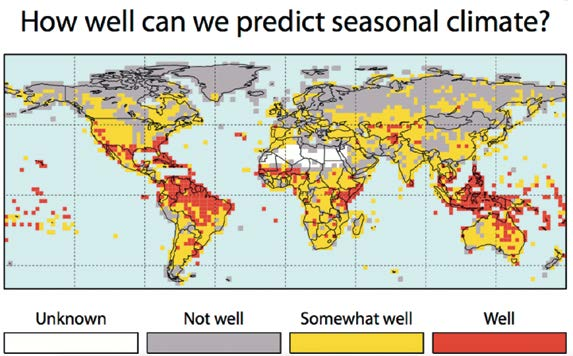
\includegraphics[scale=0.5]{REGIONS_PREDICTIBILITY.png}
    \caption*{Predictability of Regions.\footnotemark{} }
\end{figure}
\footnotetext{International Research Institute for Climate and Society}.

\section{DETERMINISTIC EVALUATION OF SEASONAL FORECAST}

	\subsection{Generalities}
In the WMO\footnotemark{} \footnotetext{https://library.wmo.int/records/item/56227-guidance-on-verification-of-operational-seasonal-climate-forecasts}. Guide, several criteria are provided for evaluating a good forecast. Each criterion offers insight into specific aspects of the model but cannot, on its own, fully determine the forecast's quality. By combining all the criteria, we can comprehensively assess the performance of the model.	 
		\subsubsection{Resolution}
	Resolution measures whether the outcome differs given different forecasts, while discrimination measures whether the forecasts differ given different outcomes.

Discrimination looks at how well your forecast separates cases when the event (outcome) happens (pass) from when it doesn’t happen (fail). It’s about telling apart the events.
Resolution looks at how well your forecast adapts to different situations, giving distinct probabilities for different cases. It’s about adjusting to the situation.

Resolution measures how well a forecast distinguishes between different outcomes. A forecast has high resolution if the predicted probabilities vary significantly depending on the actual outcome. In other words, resolution tells us whether the forecast changes (e.g., gives different probabilities) when the actual outcome changes.
High resolution: The forecast gives distinct and varying probabilities when different events (outcomes) occur. For example, if in one case the forecast predicts a high probability of rain and it rains, and in another case predicts a low probability and it doesn’t rain, the forecast shows good resolution.
Low resolution: If the forecast probabilities don’t change much regardless of whether it rains or not (e.g., always predicting a 50\% chance of rain), the forecast has poor resolution because it fails to capture the differences in actual outcomes.
Resolution can be determined by measuring how strongly the outcome is conditioned upon the forecast.
If the outcome is independent of the forecast, the forecast has no resolution and is useless
Forecasts with no resolution are neither “good” nor “bad”, but are useless. 
Metrics of resolution distinguish between potentially useful and useless forecasts, but not all these metrics distinguish between “good” and “bad” forecasts.

The following equation represents the "resolution" component of the Brier Score (BS) decomposition, which quantifies how well a set of probability forecasts differentiates between events and non-events:

\begin{equation}
\textbf {Resolution} = \frac{1}{n} \sum_{k=1}^{d} n_k \left( \bar{y}_k - \bar{y} \right)^2
\end{equation}

where:

\begin{equation}
\bar{y}_k = \frac{1}{n_k} \sum_{i=1}^{n_k} y_{k,i}
\end{equation}

\begin{itemize}
    \item $n$ is the total number of forecasts,
    \item $d$ is the number of discrete probability bins,
    \item $n_k$ is the number of forecasts in the $k$-th bin,
    \item $\bar{y}_k$ is the observed relative frequency for the $k$-th probability bin,
    \item $\bar{y}$ is the overall observed relative frequency.
\end{itemize}

The term $\left( \bar{y}_k - \bar{y} \right)^2$ captures the variance between individual forecast categories and the overall event frequency. Higher resolution indicates that forecasts better differentiate between events and non-events.



		\subsubsection{Discrimination}

Discrimination measures how well the forecast separates cases where the event occurs from cases where it does not. In other words, it examines whether the forecast probabilities differ for events that happen versus those that don't.
High discrimination: A forecast has high discrimination if, for example, when rain occurs, the forecast consistently predicts a high probability of rain, and when rain doesn’t occur, it predicts a low probability. It means the forecast is good at distinguishing between rain and no-rain days.
Low discrimination: If the forecast provides similar probabilities regardless of whether it rains or not (e.g., predicting a 60\% chance of rain every day), it has poor discrimination because it doesn’t effectively differentiate between days with and without rain.
		\subsubsection{Reliability}

A forecast is reliable if the predicted probabilities match the actual frequencies. For instance:
If you forecast a 40\% probability for below-normal rainfall, below-normal rainfall should occur in 40\% of the cases where you make that prediction.
Similarly, if you forecast a 25\% chance of above-normal rainfall, above-normal rainfall should happen 25\% of the time when you give that probability.
If this relationship holds consistently over many forecasts, the forecasts are well-calibrated (or reliable).
A Reliable but Uninformative Forecast
A forecast that always gives the climatological probability (e.g., always predicting a 33\% chance for each category: below, normal, above normal) would be reliable because the climatological average matches the observed frequencies. However, this forecast wouldn’t provide any information about changing conditions from case to case—it doesn’t adapt to the current situation, making it uninformative.

\begin{equation}
\textbf{Reliability} = \frac{1}{n} \sum_{k=1}^{d} n_k \left( \bar{p}_k - \bar{y}_k \right)^2
\end{equation}


\begin{itemize}
    \item $n$ is the total number of forecasts,
    \item $d$ is the number of discrete probability bins,
    \item $n_k$ is the number of forecasts in the $k$-th bin,
    \item $\bar{y}_k$ is the observed relative frequency for the $k$-th probability bin,
    \item $\bar{p}_k$ is relative frequency for the $k$-th probability.
\end{itemize}


		\subsubsection{Sharpness}
Sharp forecasts provide a strong signal about the expected outcome. For example, a sharp forecast might assign a 70\% chance to a certain outcome, like above-normal rainfall. This high probability communicates more confidence in that specific outcome.
On the other hand, when the forecast probabilities are close to the climatological values (like assigning a 40\% chance to above-normal, 35\% to normal, and 25\% to below-normal), the forecast is not very sharp, meaning the forecaster isn't very confident in predicting any one outcome.
The climatological probabilities are reliable, but aren’t sharp.

	\subsection{DETERMINISTIC EVALUATION.}
	First, deterministic evaluation involves calculating the anomaly, which is obtained by subtracting the climatology (the seasonal hindcast climate mean) from the forecast. The next step is to measure the correlation between the anomaly and the observed values in order to assess the accuracy of the forecast. 
	
	
	\textit{	a very important thing is that all the deterministic and probabilistic scores are available in the python package \hyperlink{https://xskillscore.readthedocs.io/en/stable/quick-start.html}{\textbf{xskillscore} }.\footnotemark{}}
	\footnotetext{https://xskillscore.readthedocs.io/en/stable/quick-start.html}
	
	\subsubsection{Correlation-Based}
	
	\begin{itemize}
	
    \item Effective Sample Size 

    \item Pearson Correlation 

    \item Pearson Correlation effective p value 

    \item Pearson Correlation p value 
 
    \item Slope of Linear Fit 

    \item Spearman Correlation 

    \item Spearman Correlation effective p value 

    \item Spearman Correlation p value 
    
    \end{itemize}

	\subsubsection{Distance-Based}
	\begin{itemize}
	
	\item Coefficient of Determination $(r_2)$

    \item Mean Absolute Error $(mae)$

    \item Mean Absolute Percentage Error $(mape)$

    \item Mean Error $(me)$

    \item Mean Squared Error $(mse)$

    \item Median Absolute Error $(median_absolute_error)$

    \item Root Mean Squared Error $(rmse)$

    \item Symmetric Mean Absolute Percentage Error $(smape)$
	
	\end{itemize}

    


	
\end{document}
